\chapter{Design}\label{chap:Design}

\section{Architektur}
\begin{figure}[h]
  \begin{center}
    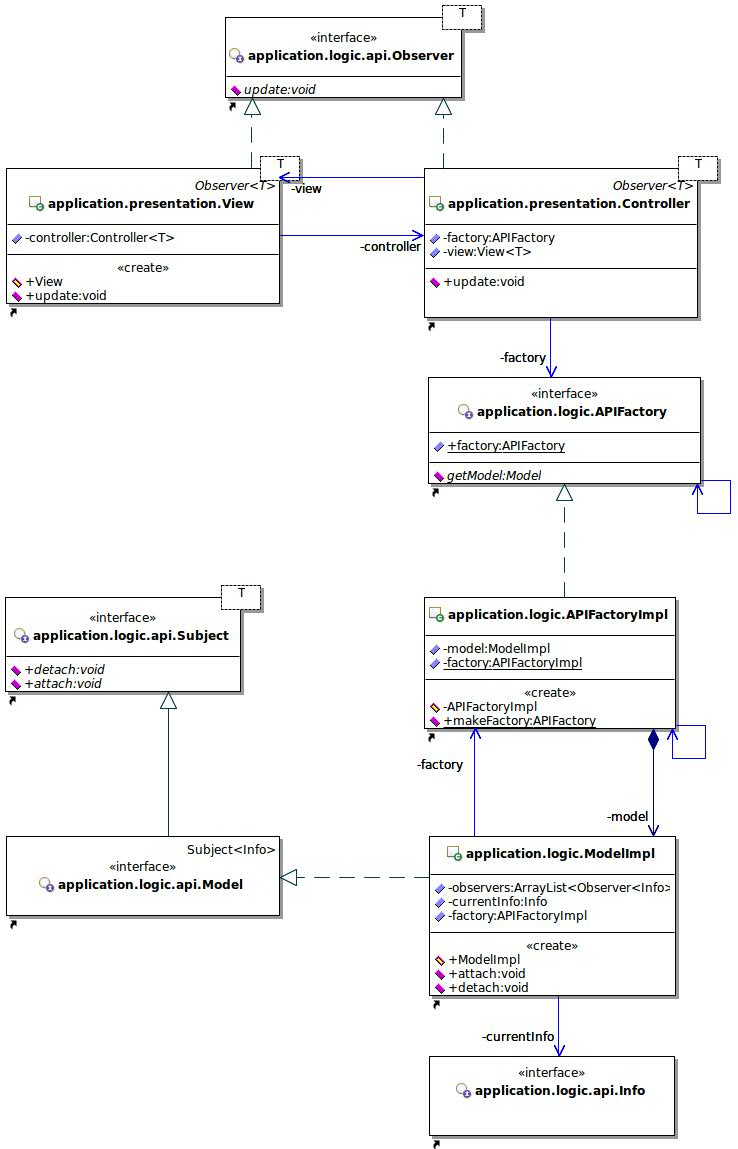
\includegraphics[width=0.6\textwidth]{diagrams/Architecture}
    \caption{Grobe Architektur des Systems}
  \end{center}
\end{figure}
\newpage

\section{Aufbereitung der Analyse und Systemoperationen}

\subsection{Mockup}
\begin{verbatim}
  Spiel wird gestartet....
  Anzahl an Spielern: 3

  Spieler Spieler 1 beginnt.

  ====
  Spieler 1 ist am Zug:

  Spieler 1: 0 von 3 Figuren im Spiel
  Spieler 2: 0 von 3 Figuren im Spiel
  Spieler 3: 0 von 3 Figuren im Spiel

  Zum Würfeln drücken Sie eine beliebige Taste: x
  Es wurde eine 3 gewürfelt.

  > Es befinden sich alle Wissensstreiter auf dem Heimatfeld - Erneut würfeln

  Zum Würfeln drücken Sie eine beliebige Taste: x
  Es wurde ein 2 gewürfelt.

  > Es befinden sich alle Wissensstreiter auf dem Heimatfeld - Erneut würfeln

  Zum Würfeln drücken Sie eine beliebige Taste: x
  Es wurde ein 3 gewürfelt.

  > Es wurde 3x gewürfelt. Der nächste Spieler ist dran

  ====
  Spieler 2 ist am Zug:

  Spieler 1: 0 von 3 Figuren im Spiel
  Spieler 2: 0 von 3 Figuren im Spiel
  Spieler 3: 0 von 3 Figuren im Spiel

  Zum Würfeln drücken Sie eine beliebige Taste: x
  Es wurde eine 6 gewürfelt.

  > Ein Wissensstreiter wurde auf das Heimatfeld gezogen

  ====
  Grün ist am Zug:

  Spieler 1: 0 von 3 Figuren im Spiel
  Spieler 2: 1 von 3 Figuren im Spiel
  Spieler 3: 0 von 3 Figuren im Spiel
\end{verbatim}

\subsection{System-Use-Case: Spielzug durchführen}
\begin{labeling}[:]{Vorbedingungen}
\item [Akteure] Model, View, Controller
\item [Priorität] Hoch
\item [Beschreibung] Nach dem das Spiel als Anwendung gestartet wurde, wird das Spiel zunächst vorbereitet. Den Spielern wird auf der Konsole mitgeteilt, welcher Spieler aktuell an der Reihe ist und wo sich seine Wissensstreiter befinden. Danach wird der aktuelle Spieler zum Würfeln aufgefordert. Er kann das Würfeln durch einen beliebigen Tastendruck auslösen, wobei dann ein Würfelergebnis zufällig bestimmt wird. Das Würfelergebnis wird ebenfalls auf der Konsole ausgegeben.
Ist das Würfelergebnis gleich 6 und hat der aktuelle Spieler noch einen Wissensstreiter auf dem Heimatfeld und  ist sein Startfeld frei, dann wird ein Wissensstreiter des Spielers auf sein Heimatfeld gestellt. Der Spieler wird darüber auf der Konsole informiert. Ist das Heimatfeld belegt startet eine Fragerunde.
Hat der Spieler alle Wissensstreiter auf dem Pfad, oder er hat eine Augenzahl kleiner als 6 gewürfelt, dann wird ihm eine Auswahlliste seiner Wissensstreiter auf der Konsole präsentiert und er kann durch Eingeben einer Nummer einen Wissensstreiter auswählen, den er versetzen möchte. Sollte der Wissensstreiter auf ein Feld kommen, welches bereits durch einen anderen Wissensstreiter belegt ist, beginnt eine Fragerunde.
Hat der Spieler eine Augenzahl gewürfelt, die kleiner als 6 ist, und hat er noch alle Wissensstreiter auf seinen Heimatfeldern, dann wird er erneut zum würfeln aufgefordert bis er 3 mal in diesem Zug gewürfelt hat.
Alle Eingaben des Spielers werden validiert. Ist eine Eingabe Fehlerhaft wird der Spieler erneut zur Eingabe aufgefordert.
Ein Spieler wird über das Ende seines Zuges auf der Konsole informiert.
\item [Vorbedingungen] Anwendung gestartet, Spiel vorbereitet
\item [Offene Punkte]
\end{labeling}

\newpage
\subsubsection{Use-Case Diagramm}
\begin{figure}[h]
  \begin{center}
    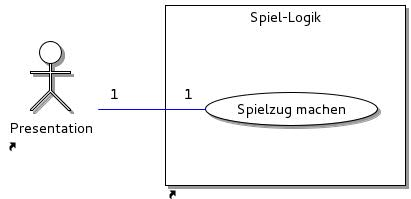
\includegraphics[width=0.8\textwidth]{design/spielzug_machen_system_usecase}
    \caption{Use-Case \"Spielzug machen\"}
  \end{center}
\end{figure}
\newpage

\subsubsection{Activity Diagramme}
\begin{figure}[h]
  \begin{center}
    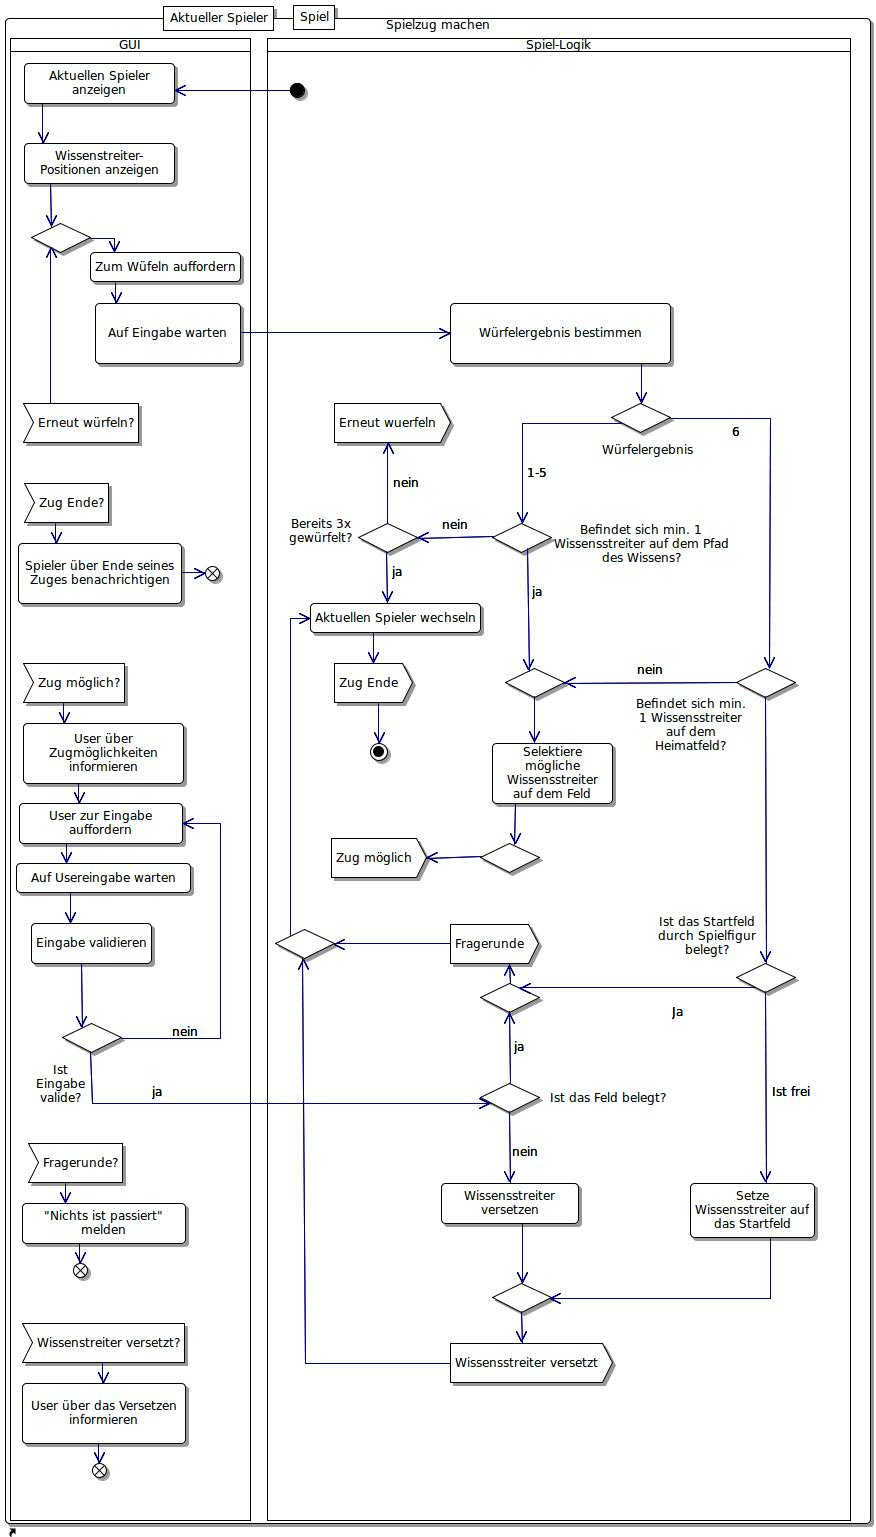
\includegraphics[width=0.6\textwidth]{diagrams/Ablauf_Spielzug_machen_10062016}
  \end{center}
\end{figure}
\newpage

\subsection{Schnittstelle der Applikationsschicht}

Was kommt hier rein?!?!?!
\newpage

\subsubsection{System-Sequenz Diagramm}

\subsubsection{Operation: würfeln()}
\begin{labeling}[:]{Verantwortlichkeit}
\item [Parameter] -
\item [Verantwortlichkeit] Es wird ein zufälliges Würfelergebnis bestimmt.

Ist das Würfelergebnis kleiner als 6 und befindet sich mindestens 1 Wissensstreiter des aktuellen Spielers schon auf dem Pfad, dann wird eine Liste mit allen Wissensstreitern des Spielers, die sich auf dem Pfad befinden, angezeigt. Der Spieler hat dann die Möglichkeit einen Wissensstreiter auszuwählen, indem er die Nummer des Wissensstreiters angibt.

Ist die Augenzahl kleiner als 6, hat der aktuelle Spieler noch nicht 3 mal gewürfelt und es befinden sich noch alle Wissensstreiter des Spielers auf den Heimatfeldern, dann wird der Spieler noch einmal zum Würfeln aufgefordert.

Ist das Würfelergebnis gleich 6 und es befinden sich noch 1 Wissensstreiter des Spielers auf den Heimatfeldern, dann wird, sofern das Startfeld frei ist, ein Wissensstreiter auf das Startfeld gesetzt. Ist das Startfeld belegt, beginnt eine Fragerunde. Danach wird der nächste Spieler ausgewählt und der aktuelle Zug beendet, was durch eine Textausgabe angezeigt wird.

Befinden sich alle Wissensstreiter auf dem Pfad, dann wird ganz unabhängig von der Augenzahl eine Liste mit allen Wissensstreitern, die vom Spieler versetzt werden können, ausgegeben.
Der Spieler hat dann die Möglichkeit einen Wissensstreiter auszuwählen und zu versetzen.
\item [Ausnahmen]
\item [Vorbedingungen] Es gibt einen aktuellen Spieler und der Spieler hat noch nicht 3 mal gewürfelt.
\item [Nachbedingungen] Der Spieler kann einen Wissensstreiter versetzen, oder erneut würfeln, oder es wurde ein Wissensstreiter des Spielers von den Heimatfeldern auf sein Startfeld gezogen bzw. deswegen eine Fragerunde gestartet. Sein Zug ist bei dem letzten Fall dann beendet, sowie der nächste Spieler ist ausgewählt.
\end{labeling}

\subsubsection{Operation: versetzeWissensstreiter(Wissensstreiter)}
\begin{labeling}[:]{Verantwortlichkeit}
\item [Parameter] Ausgewählter Wissensstreiter
\item [Verantwortlichkeit] Ist das Feld auf das der Wissensstreiter gezogen werden soll frei, dann wird er auf dieses Feld gezogen. Ist das Feld belegt beginnt eine Fragerunde.

Nach dem Versetzen oder der Fragerunde wird der Spieler gewechselt und der aktuelle Zug beendet. Das Ende des Zuges wird dem mit einer Nachricht die ausgegeben wird signalisiert.

\item [Ausnahmen]
\item [Vorbedingungen] Der aktuelle Spieler hat einen Wissensstreiter ausgewählt und die Eingabe ist valide. Es existiert eine vom Spieler zuvor gewürfelte Augenzahl.
\item [Nachbedingungen] Der Wissensstreiter wurde versetzt oder eine Fragerunde begonnen. Der nächste Spieler wurde ausgewählt und der Zug des aktuellen Spielers beendet.
\end{labeling}

\section{Zustandsautomaten}
\begin{figure}[h]
  \begin{center}
    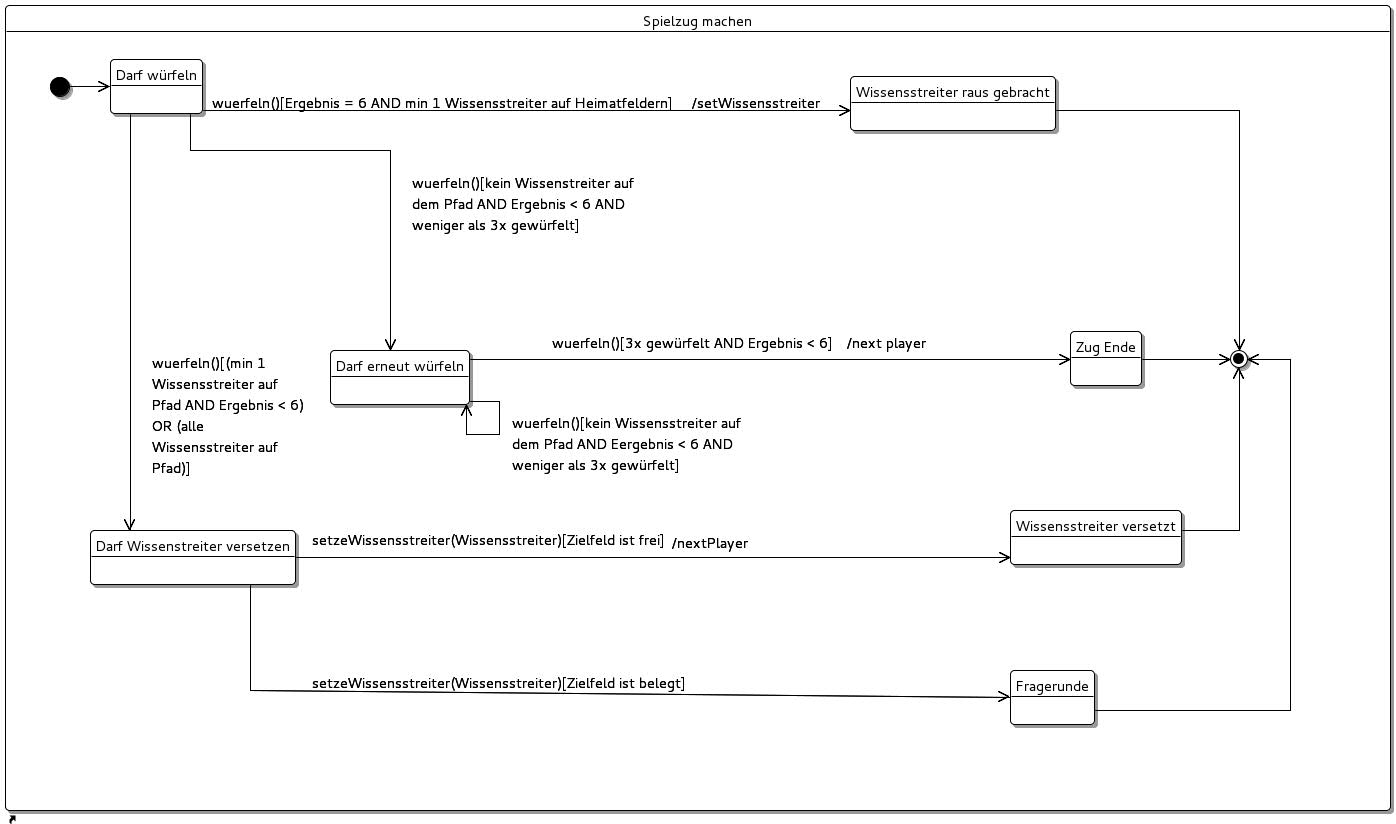
\includegraphics[width=0.95\textwidth]{design/spielzug_machen_state_machine}
    \caption{Zustandsautomat für Use-Case \"Spielzug machen\"}
  \end{center}
\end{figure}
\newpage

\section{Detailed Design und das Objektmodell}
\subsection{Sequenz- und Kommunikationsdiagramm}
\begin{figure}[h]
    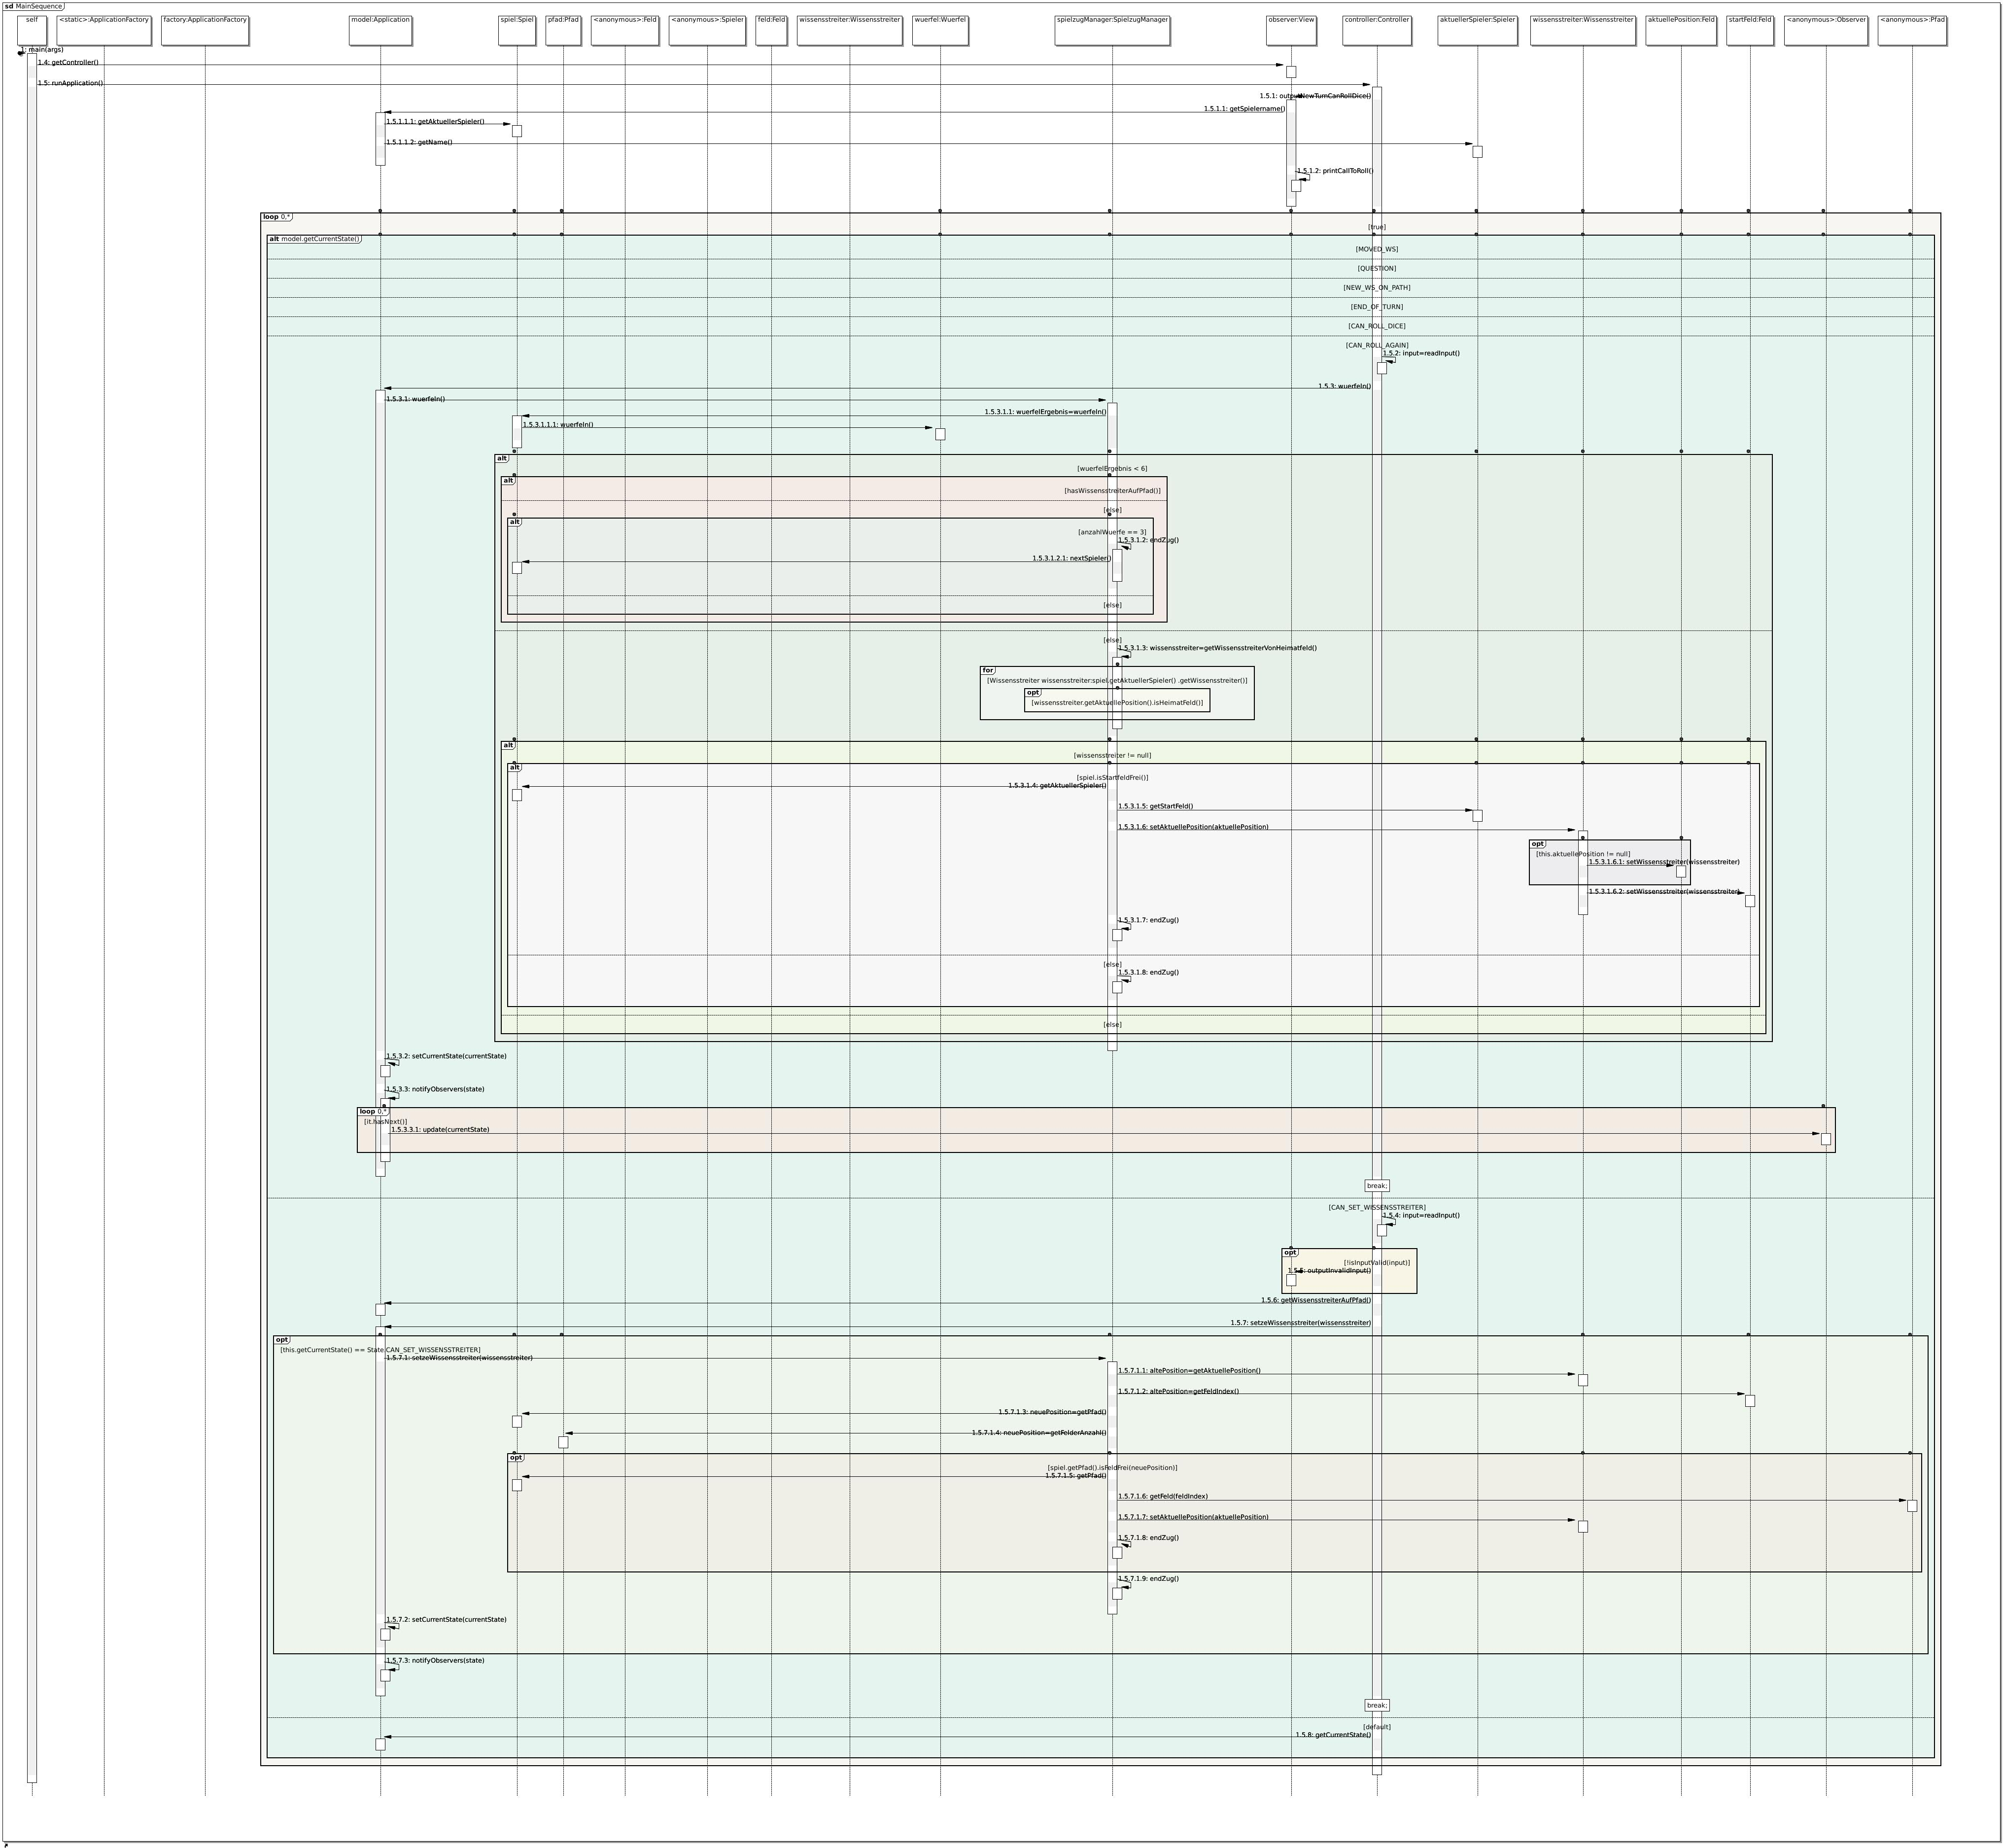
\includegraphics[width=1.1\textwidth]{design/MainSequence}
    \caption{Das \texttt{Main} Sequenz Diagramm}
\end{figure}
\newpage
\begin{figure}[h]
  \begin{center}
    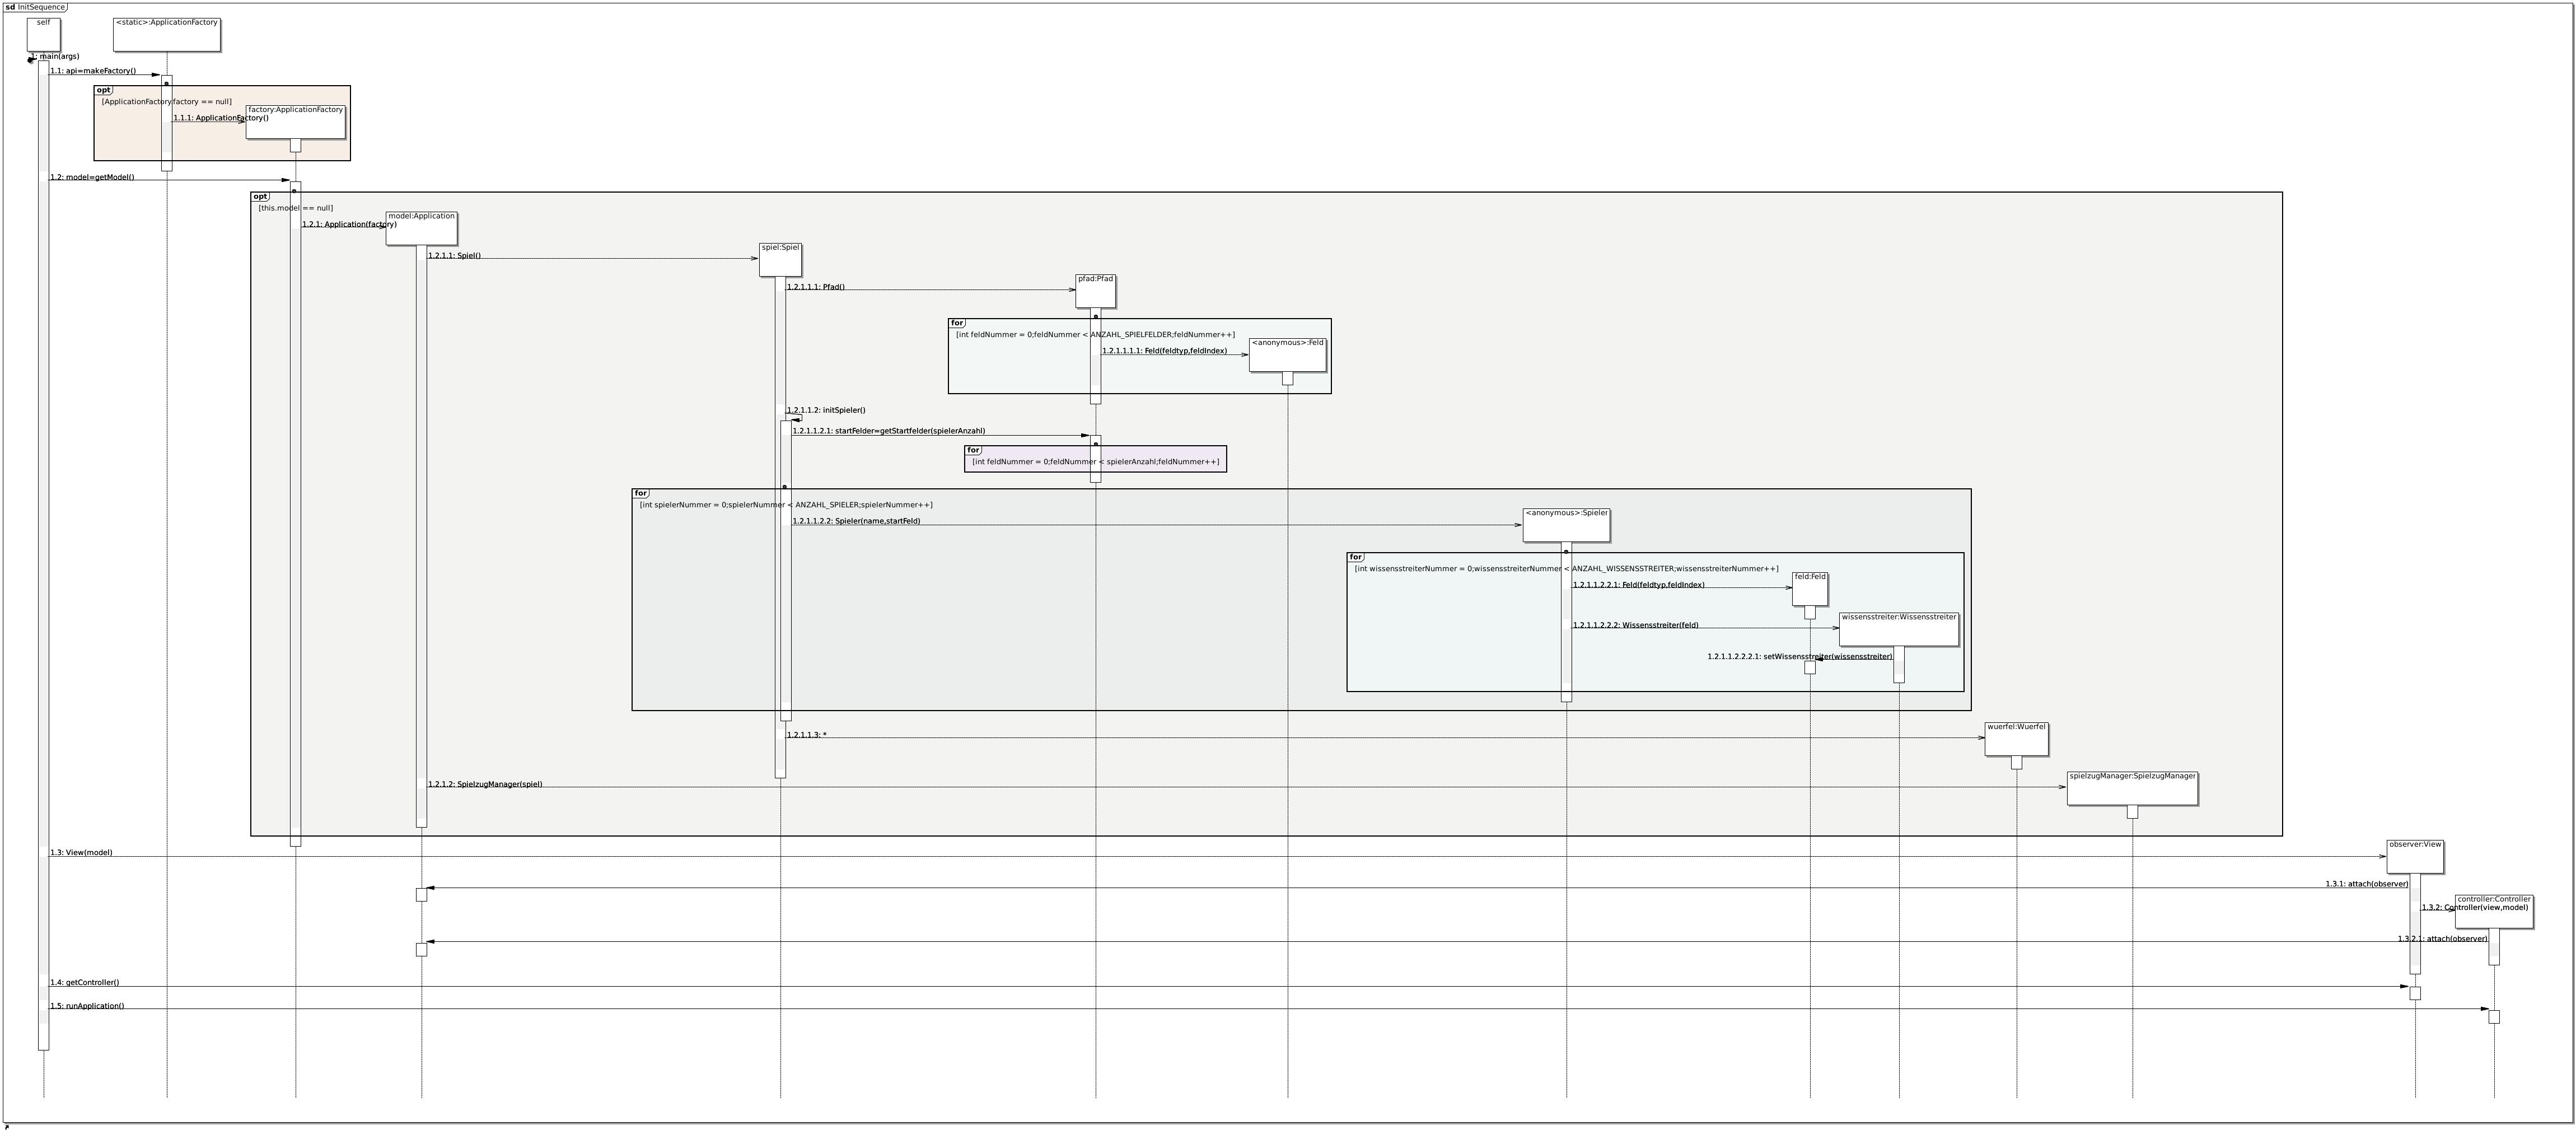
\includegraphics[width=1.1\textwidth]{design/MainInitSequence}
    \caption{Das \texttt{Main Init} Sequenz Diagramm}
  \end{center}
\end{figure}
\newpage


\subsection{Design-Objektmodeel}
\begin{figure}[h]
  \begin{center}
    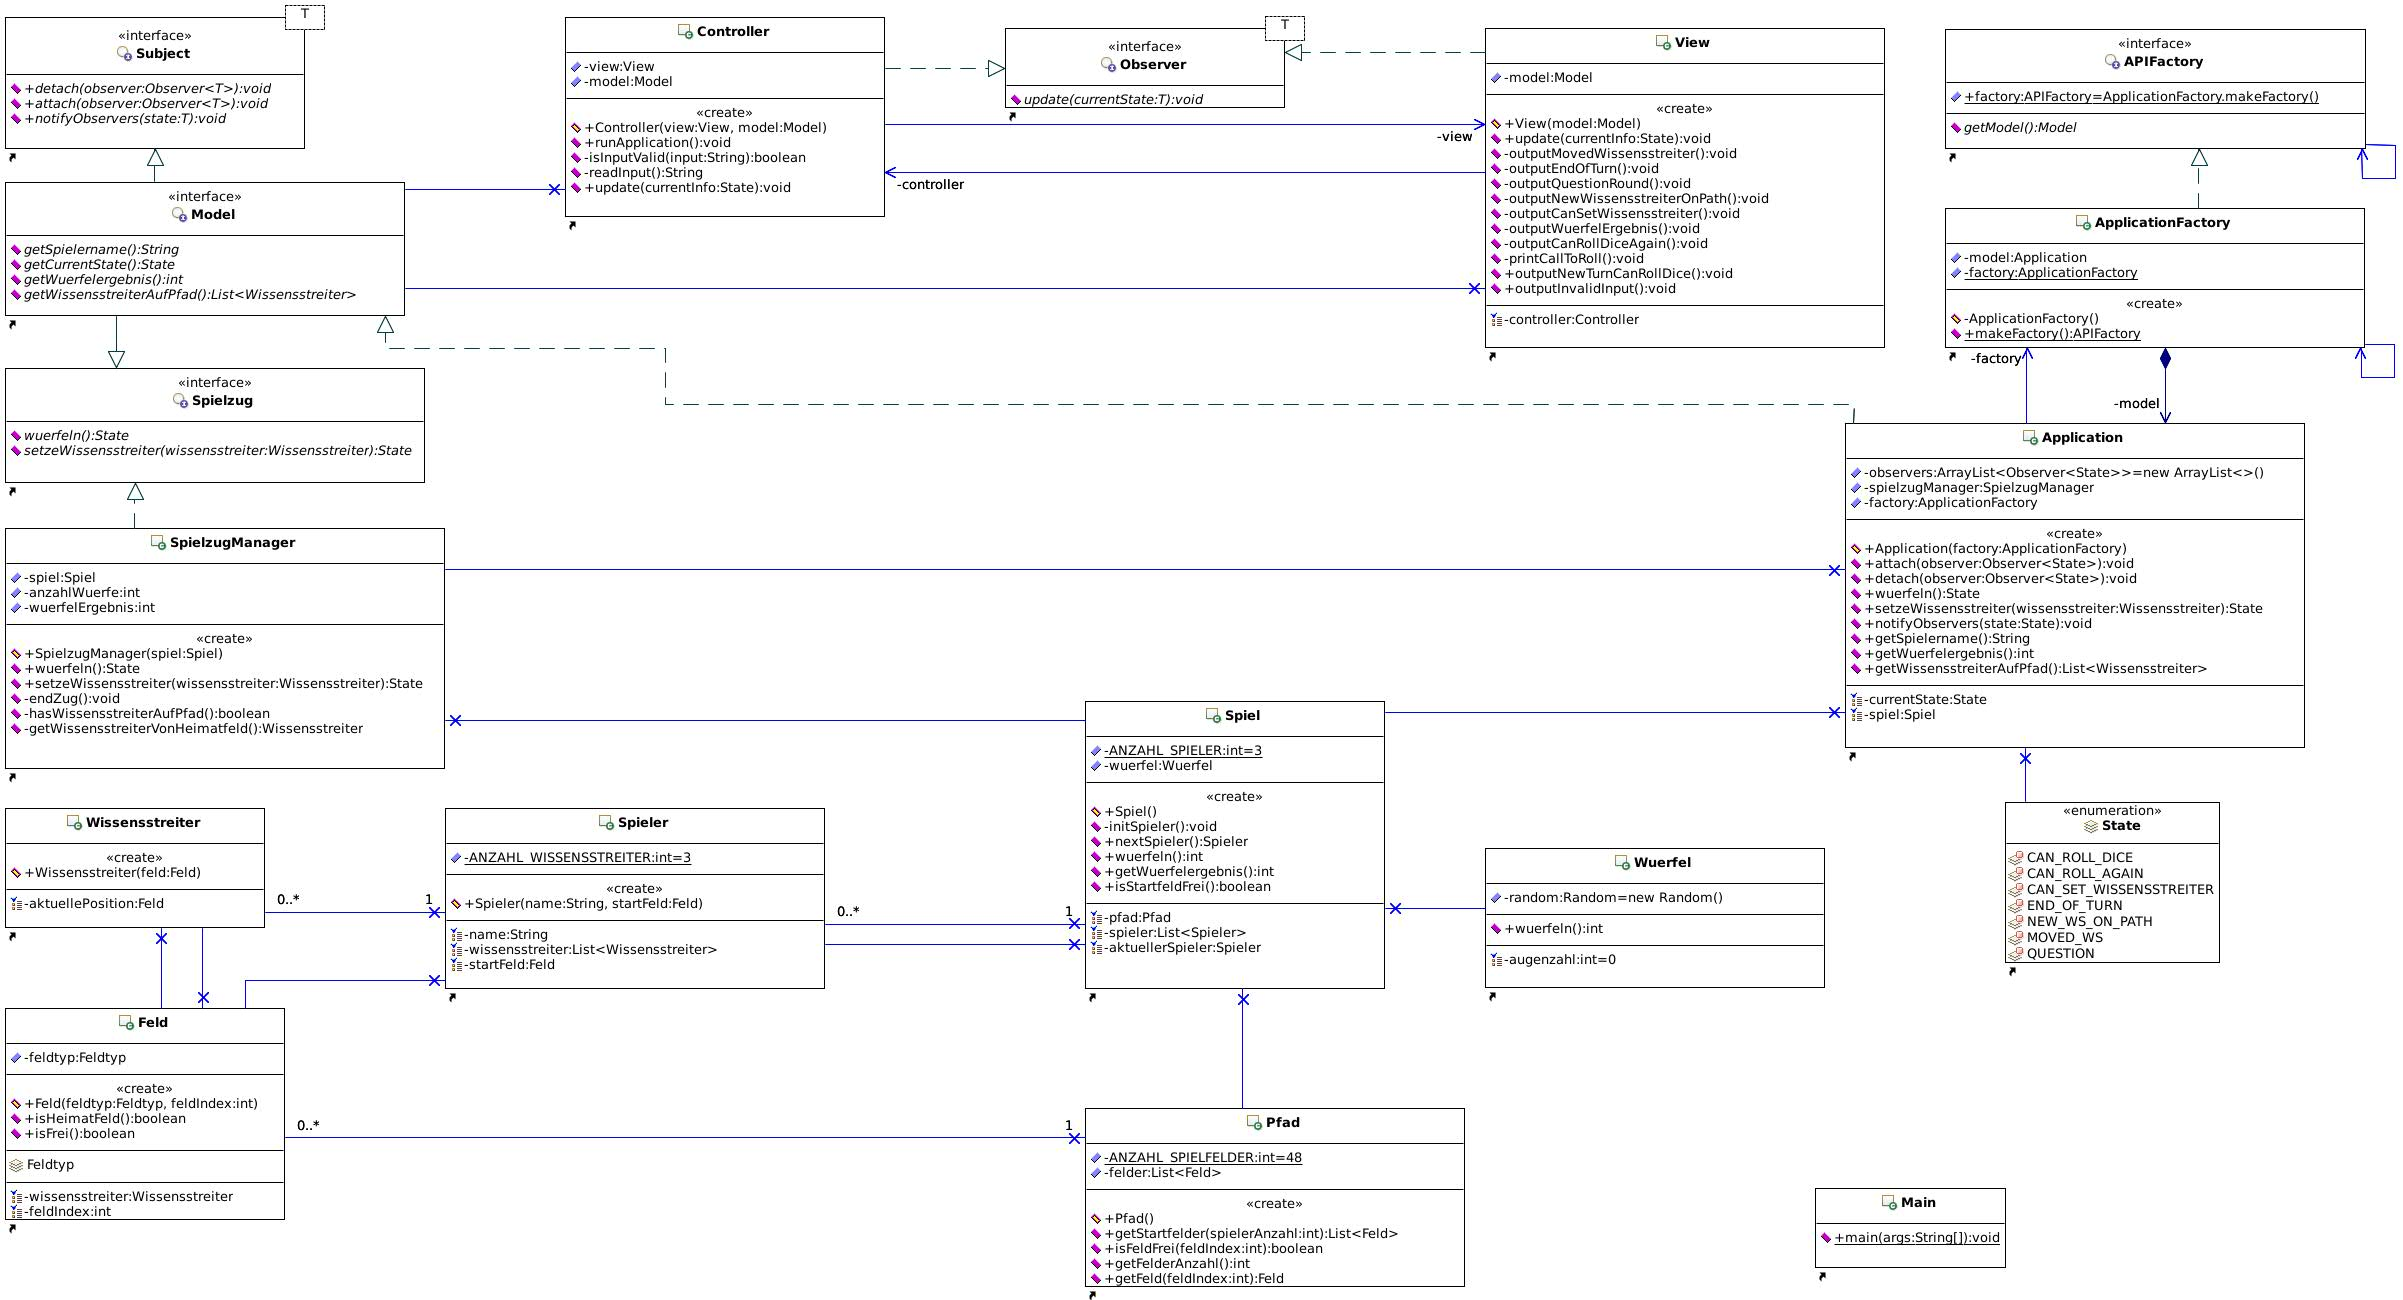
\includegraphics[width=1\textwidth]{design/ClassObjectDiagram}
    \caption{Das Klassen-Objekt-Diagramm}
  \end{center}
\end{figure}
\newpage

\section{Implementierung der Oberfläche}
Die Implementierung kann man dem abgegebenem Jar Programm entnehmen.
